\documentclass[10pt,a4paper]{article}

\usepackage{main}
\usepackage{exercices}

\renewcommand{\typedocument}{Exercices}
\renewcommand{\classe}{3e}
\renewcommand{\titre}{Révision Brevet}

\renewcommand{\exercice}[1]{%
    \refstepcounter{numexercice}%
    \vspace{0.5em}%
    \noindent
    {\large \textbf{\thenumexercice{}. #1}}%
    \par
    \vspace{0.1em}%
}

\begin{document}

\begin{multicols*}{2}

\exercice{Mission Sentinel-6A (Métropole 2023)}

\textbf{Principe de l'altimétrie radar par satellite}

\begin{center}
    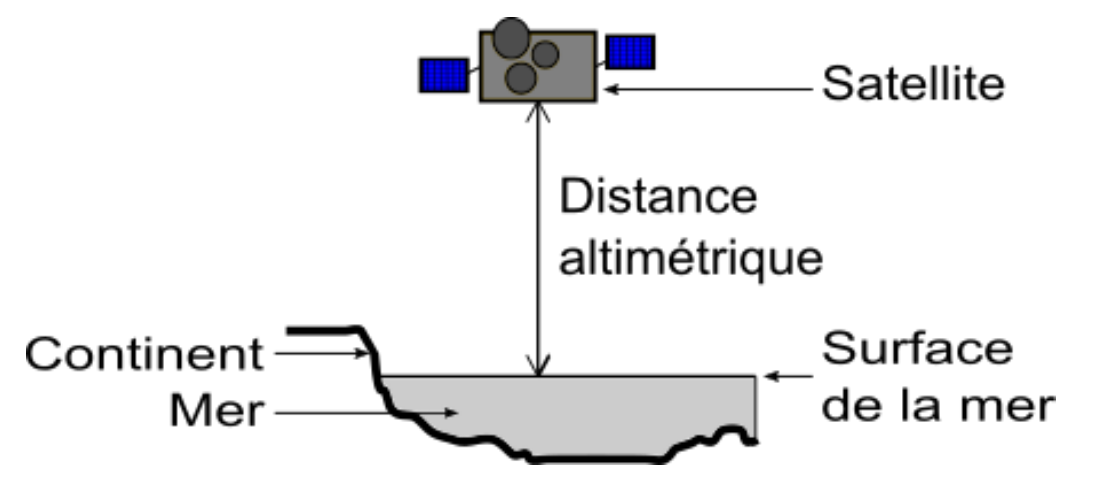
\includegraphics[width=0.6\linewidth]{images/3A6X_1.png}
\end{center}

Afin de déterminer le niveau marin, le satellite mesure la distance altimétrique, c'est-à-dire la distance entre le satellite et la surface de la mer. Un radar, embarqué sur le satellite, émet verticalement des ondes radio, sous forme de signaux de très courtes durées. Ces signaux, qui se propagent à la vitesse de 300 000 km/s, se réfléchissent sur la surface de la mer, reviennent jusqu’au satellite et sont détectés par l’antenne du radar. La durée mise par un signal radio pour faire l’aller-retour permet de déterminer la distance altimétrique.

\question{Déterminer la valeur de la distance altimétrique mesurée par le satellite Sentinel-6A lorsque le signal met 8,9 ms (soit 0,0089 s) pour effectuer l'aller-retour entre le satellite et la surface de la mer. Expliquer la démarche. Préciser la relation utilisée et commenter le résultat obtenu.}

\exercice{Sécurité électrique à bord d'un voilier (Asie 2025)}

Un voilier moderne doit être équipé d'une installation électrique efficace, et fiable afin de permettre le bon fonctionnement des équipements de sécurité, de navigation et de confort. Ces appareils fonctionnent indépendamment les uns des autres.

À bord de la plupart des voiliers, une batterie 12 V fournit l'énergie électrique nécessaire à tous les appareils.

\question{Préciser si les appareils récepteurs dans le voilier sont branchés en série ou en dérivation et justifier la réponse.}

Une lampe tricolore est placée à l'avant du voilier. Elle peut être modélisée par une lampe de puissance nominale 6 W et de tension nominale 12 V.

La tension nominale de la lampe est la tension à laquelle elle doit être soumise pour qu'elle brille normalement.

\question{Montrer par un calcul que la valeur de l'intensité du courant dans le fil d'alimentation de la lampe tricolore est égale à 0,5 A quand cette lampe fonctionne normalement.}

Sur le voilier, la lampe tricolore brille très faiblement, car le fil de cuivre d'une des connexions qui relie cette lampe à la batterie de tension 12 V s'est oxydé.

Le circuit électrique qui modélise la situation est alors équivalent au montage ci-dessous. Le fil de cuivre oxydé y est modélisé par une résistance en série de valeur 47 \si{\ohm}. La valeur de l'intensité mesurée dans le circuit est égale à 0,19 A. 

\begin{center}
    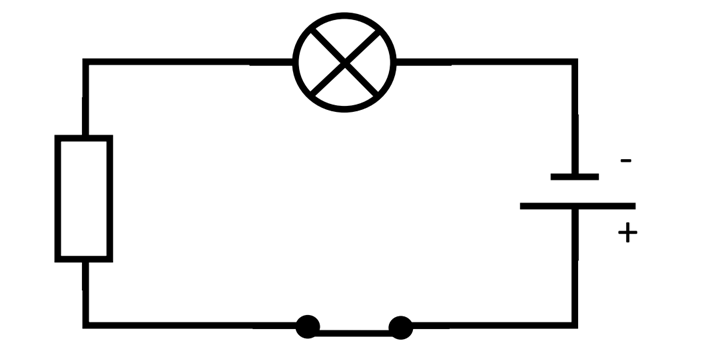
\includegraphics[width=0.5\linewidth]{images/3A6X_2.png}
\end{center}

\question{Recopier le schéma du circuit ci-dessus sur votre copie en ajoutant les schémas normalisés des appareils permettant la mesure de la tension aux bornes de la résistance et de l'intensité du courant qui la traverse.}

\question{Rappeler quel est l'effet de l'ajout d'une résistance électrique sur la valeur de l'intensité du courant dans un circuit en série.}

Lorsqu'elle est traversée par un courant d'intensité de valeur égale à 0,19 A, la tension aux bornes de la résistance est égale à 9 V.

\question{On considère que la tension aux bornes de l'interrupteur fermé est nulle. Déterminer la valeur de la tension aux bornes de la lampe. Commenter le résultat.}

\exercice{Météorites (Nouvelle-Calédonie 2021)}

Lorsqu’une météorite pénètre dans l'atmosphère terrestre, les frottements avec l'air provoquent son ralentissement et son échauffement. Elle se transforme alors en boule de feu qui finit par se fragmenter en petits morceaux.

\question{Calculer la valeur de l'énergie cinétique Ec d'une météorite d'une masse de 80 000 kg qui entre dans l'atmosphère à la vitesse de 12,8 km/s. Détailler le calcul réalisé.}

\question{Indiquer comment évolue l'énergie cinétique Ec lorsque la météorite pénètre dans l'atmosphère terrestre. Justifier la réponse.}

\exercice{Circuit électrique de fourgon (Groupe 1 2020)}

On modélise l’installation électrique d'un fourgon par le circuit schématisé ci-dessous.

\begin{center}
    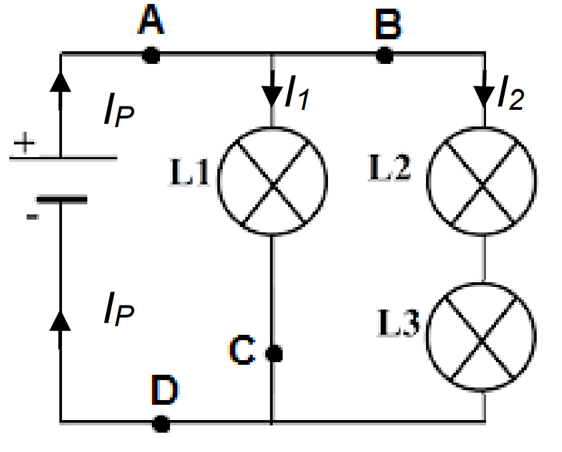
\includegraphics[width=0.5\linewidth]{images/3A6X_3.png}
\end{center}

\question{On souhaite ajouter dans le circuit un interrupteur capable d’allumer et d’éteindre toutes les lampes en même temps. Indiquer, parmi les positions A, B, C ou D où pourrait être placé l’interrupteur pour répondre à ce cahier des charges.}

Lorsque toutes les lampes sont allumées, la pile a une tension électrique à ses bornes U = 12 V.

À l’aide d’un ampèremètre, on réalise plusieurs mesures :

\begin{itemize}
    \item intensité du courant électrique dans la branche principale I\textsubscript{P} = 0,15 A
    \item intensité du courant électrique traversant les lampes L2 et L3 I\textsubscript{2} = 0,12 A.
\end{itemize}    

L’aménagement ne permettant pas de mesurer directement l’intensité I\textsubscript{1} du courant électrique traversant la lampe L1, on cherche à obtenir sa valeur par un calcul.

\question{Vérifier, en justifiant la réponse, que la valeur de l’intensité I\textsubscript{1} du courant électrique traversant la lampe L1 est égale à 30 mA.}

\question{Sur la lampe L1 figurent les indications suivantes : 12 V ; 0,36 W. Justifier que la lampe L1 fonctionne dans les conditions normales d’utilisation.}

\end{multicols*}
\end{document}
